\chapter{Data format and Adjoint Tomography Workflow}
\label{ch:tools}

\section{Introduction}

Seismology is a scientific discipline driven by data.
Seismological research usually involves the process
of observing, modeling, and understanding seismographic data.
In our first-generation
global tomographic FWI model, we used a database of 253 earthquakes. In our second-generation
model, which is the main topic of this thesis, the dataset was gradually
increased to 1,480 earthquakes, and great improvements started to
emerge in our model.
In the process of constructing the new model, we have overcome various technical
challenges which we cover in this chapter.
It will become obvious that these efforts not only enabled research progress,
but are an absolute necessity for further upscaling the tomographic inversions.

Global adjoint tomography not only relies on advanced
numerical methods and top-tier computer hardware, but is also subject to 
rapid developments in the software infrastructure.
This chapter covers three such challenges.
We first discuss our efforts to develop a new seismic data format,
which facilitates calculation efficiency
and data integrity.
We then discuss building more efficient
and robust software, using the data processing workflow as an
example.
Finally, we discuss how to integrate each component of the modeling and inversion process
into a complete workflow management system.


\section{Data format}

With the growth of our earthquake database, challenges comes from two directions.
First, SPECFEM3D GLOBE is a spectral finite element solver that heavily
relies on the mesh of the input model.
The mesh file not only stores
the position and physical properties of the GLL points, it also stores
the kernel and gradient information on associated points. Given our current
resolution at 17~second, each forward simulation will generate ~60GB mesh
files and ~12GB kernel files. However, the undo-attenuation has brought this
problem into a whole new level. In order to calculate the kernels in the adjoint
simulation with attenuation effect, SPECFEM will save the forward wavefield,
to be later used in the wavefield reconstruction in the adjoint stage.
Given our current resolution,
it will generate ~1TB of wavefield files in the forward simulation, and those
files needed to be dumped and saved on the disk for later use in adjoint simulations.
Thus, given the current size of dataset,
1,480 earthquakes will in total created ~1.5PB files in about 6~hrs simulations.
This posed huge challenges into the file system and we have seeking for
a efficient data container to solve the problem. ADIOS, developed by Oak Ridge
National Lab, is selected as the data container to save the mesh data.
In the Appendix ~\ref{subsection:ADIOS}, we will discuss in detail about it.
However, given the current 1,480 earthquakes and resolution at 17~sec,
there are already 1.5PB files saved to the file system. In the future, we are
planning to push to 6,000 earthquakes and resolution at 9~sec, the mesh files
will be at least 30 -- 50 times larger than the current data size. There is no file
system could handle such massive I/Os in such a short simulation time. Even
the file system can handle it, the file saving operation would be extremely 
expensive. Source-encoding might be potential technique to avoid saving the forward
wavefield files, which is major portion of the I/O loads.

Other than the mesh data, seismic data also scales linearly with the number
of earthquakes. Unlike mesh data, seismic data, contains various different
data types including earthquake source, waveform and station data.
Earthquake source describes the source mechanism. There are many standard
format to store the source information, such as NDK, CMTSOLUTION, QuakeML and etc,
among which QuakeML is the most versatile source format thanks to its flexible
internal structure.

Waveform data, which is the time series data recording the ground motion, takes
the most of the storage space.
There are also many standard data format that are used to store the waveform
data. The most commonly used ones including SAC and MSEED. For example, the SAC format
will store the time series data, together with meta data
in its pre-defined header slots. The meta data contains very limited information
which compliment the time series, such as the start time, sampling rate, station
information, such as station location and instrument orientations. It becomes quite
handy when processing small batch of data, but becomes really cumbersome processing
large volumes of data, for reasons we mentioned below.

The last one is station information, including the station location, component orientation,
instrument response and etc. The station location information are used to calculate the 
azimuth and back-azimuth, future to rotate the seismograms. The orientations are used
to check the integrity of the data in our workflow, whether the North and East component are installed
orthogonal and correctly pointing to the right direction. The instrument response
file will used to remove the instrument response and recover the true ground motion
in the data processing stage. RESPs and Pole-Zeors files are among the standard
format to store the response information(but it can only store the response data).
StationXML is a more comprehensive data format that keeps all the station information
and becomes more and more popular now days.

It is obvious to see that there are intrinsic differences between the model and seismic data.
For model files, the data structure are relatively homogeneous. They are mostly
array-like data, even though there are multiple arrays belonging to different physical
properties. Despite the simple data structure, as the mesh data volumes reaches petabytes level,
the data container should provide us with the best performance
and efficiency. That's why we used ADIOS since it is mainly optimized for those
factors.

On the other hand, seismic data is very heterogeneous. Even
though the data volume is not so large compared to model files, it is very crucial to
keep everything in a ordered and structured manner. For example, 
waveform data has to be associated with its own source and stations. If the wrong
event or station files are used, it will generate contamination in our results.

With thousands of earthquakes and millions of seismic traces, it is crucial for
us to find the right way to maintain the integrity of seismic data.
In our first-gen model, we used CMTSOLUTION to store the source information and each
CMTSOLUTION file contains one source. SAC format is used to store waveform data and
RESP to store the instrument response information. It really becomes a huge challenges
when we scale our dataset up since each SAC can only store one time series and so
does RESP file. Given 1,480 earthquakes, the time series data can easily scale up to millions
of traces and response files, bringing the high-performance computer and file system
into its knees with such a large number of I/O request, over and over again.
Also, maintaining the relationship between data are kept externally using directories
in the file system,
which is fragile and error-prone since directories can be easily manipulated.
All the factors mentioned above drove us to
look for a new data format that satisfy the needs for modern seismic data processing.
In collaboration with Oak Ridge National Lab and Lion Krischer, we introduced the 
ASDF. The typical usage of ASDF in our workflow is to store all the data from one
event. So a single ASDF file will contains not only all the seismic traces from one
event, but also associated source(QuakeML) and station information(STATIONXML).
In one data processing stage, we only need the ASDF without the need to reach out
external files. ASDF not only improves the data integrity, but also processing efficiency.
With the functional programming, ASDF can take user-defined function and dispatch the job
in a parallel manner. For most of the computational intensive steps, such as signal
processing, window selection and etd, we are using the parallel functions in ASDF
to facilitate our processing speed.
For More details about ASDF, please refer to the Appendix ~\ref{chapter:asdf}.


\section{Data Processing Workflow and Tools}
\label{section:data_processing}

Other than the data format itself, it is also crucial to build new software
to fully take advantage of it.
Fig.~\ref{fig:preprocess_workflow} shows the data processing workflow.
In our first-gen model, SAC software was used in the signal processing part.
FLEXWIN and Measure\_Adj were used in the window selection and measurements part
(including measurements and adjoint source calculation).
Those two packages are originally written in Fortran. For fully accommodate
and utilize the new  data format, we re-build all of software into python,
due to following reasons mentioned below.

\subsection{Data Processing Workflow}
\begin{figure}
  \centering
  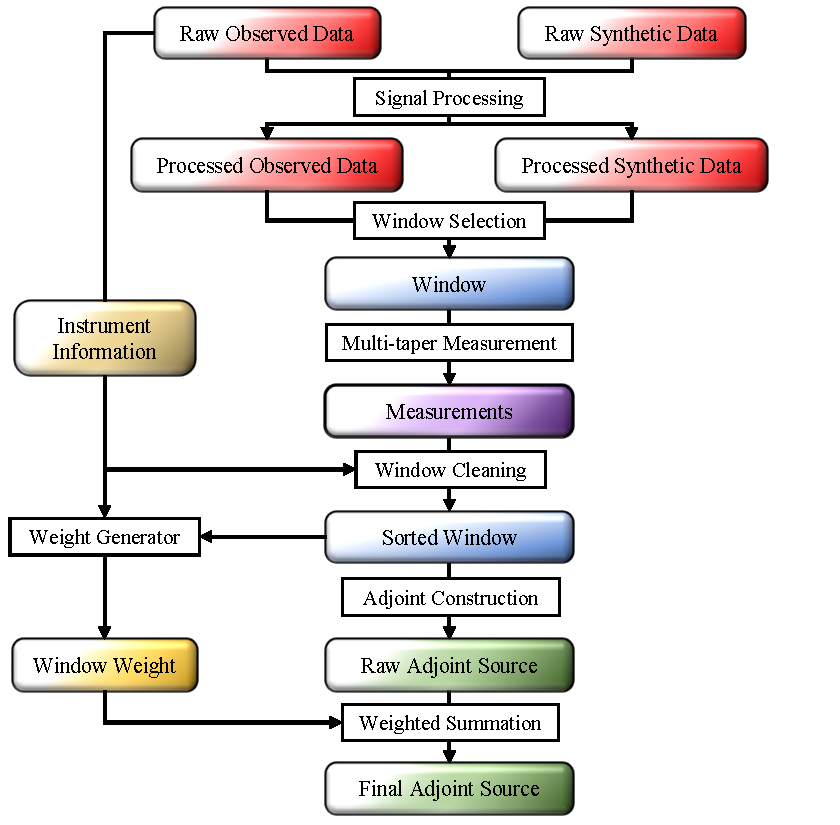
\includegraphics[width=0.8\textwidth]{ch-GLADM25/figures/Preprocess_workflow.pdf}
  \caption[Sub-workflow workflow for pre-processing seismic data]
  {\small{Sub-workflow workflow for pre-processing seismic data.}}
  \label{fig:preprocess_workflow}
\end{figure}

First, python provides great community and open-source support, meaning for most
of the lower level implementation we don't need write the code but
just find the right python library. For example,
The Numpy and Scipy provide common numerical and matrix operations.
Obspy is a seismic data analysis toolkit, implemented
most of the functions we used in the signal processing stage, such as taper, filtering
and instrument response. It is more powerful than SAC,
providing more rich APIS, such as support for more versatile I/O methods, reading
various source(such NDK, CMTSOLUTION and QuakeML), station(RESP, Pole-Zeros, STATIONXML)
and seismic data(SAC, MSEED, SEGY and etc) format.
Also, for ASDF, we used HDF5 as the underlying data container, which already has
stable python libraries, h5py, to read and write HDF5 files in serial or parallel manner.

Second, it is very easy to develop our processing tools in a modular style with python.
Integration of open-source python packages, such as Numpy, Scipy and Obspy take much
less effort than Fortron or C due to its dynamic language features.
Thanks to the very powerful python software management system,
about maintaining integrity of external python libraries, using pip and Ananconda.
Those tools also comes with version control capability,
For Fortran and C software, external libraries
are usually needed to be packed with the software itself. It not only increased the size
of the packages, but also requires users to maintain the libraries themselves. It will
 soon becomes a nightmare when the software has a lot of external dependencies.

There are definitely disadvantages using python. The most known issue people criticize is the
efficiency of python language due to its dynamic nature.
It would never reaches the performance
as static-compiled language like C or Fortran. However, for the data processing workflow,
there are many factors that are more critical than language efficiency, such as fast
development, easy deployment and user-friendly. It is also obvious that python
has gained so much popularity the in data science and machine learning domain, where
people extensively relying on the python language and libraries to processing big data.

Nevertheless, it is not saying efficiency is not important for data processing
given that we still have millions of seismograms to process in each iterations.
For lower level python libraries, such as Numpy, it is written in C but
providing user's with python interface for numerical intensive operations.
For basic array and matrix operations, it can reaches
almost the same performance as static languages. For higher-level python software
we build, parallel processing is very easily achieved using the python APIs in ASDF.
In the following, we will focus on the software we developed
 for the data processing workflow.

\subsection{Software}

\begin{figure}
  \centering
  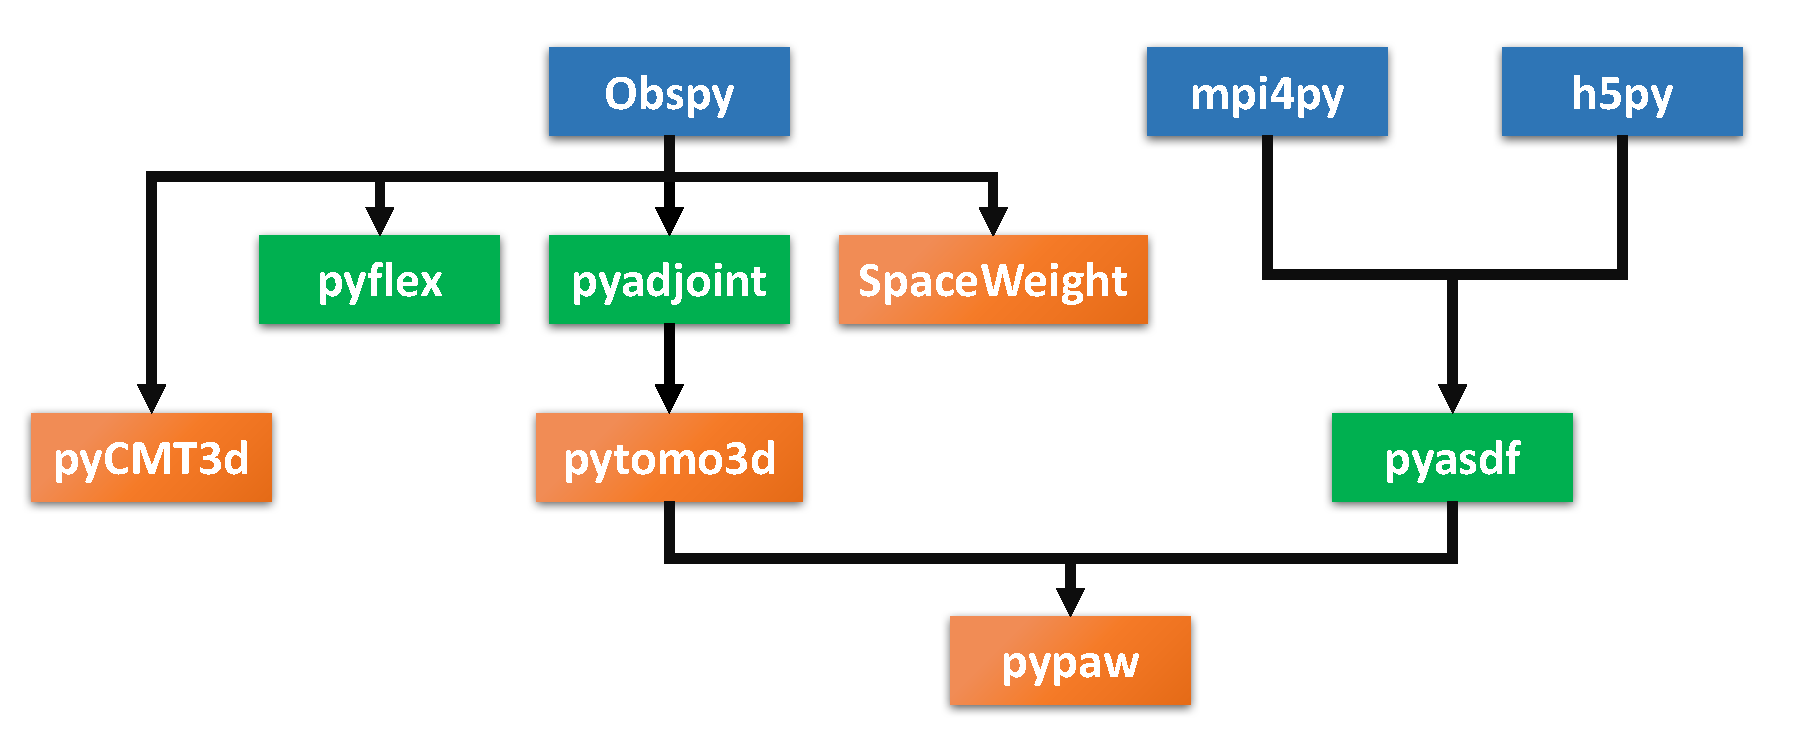
\includegraphics[width=0.98\textwidth]{ch-tools/figures/data_processing_software.pdf}
  \caption[software built for pre-processing seismic data]
  {\small{Software built for pre-processing seismic data. The position and arrows denotes
  the dependency of software. The color denotes the contribution level. Software with
  orange box denotes I am the major developer of the packages, while Greens mean I have
  contribute to and Blue are common open-source libraries (there are many open-source
  libraries we used but only major ones are listed.). We do keep all of our software
  open-source as well.}}
  \label{fig:preprocess_software}
\end{figure}


Fig.~\ref{fig:preprocess_software} shows the software tree we developed
for the seismic data processing workflow.

Obspy is sitting at the lowest level at the processing branch. It provides
APIs for operations on time series data. It is also used in
parsing for QuakeML and StationXML files, calculation of arrival time, azimuth,
sta-lta, component rotation and etc.

At the second level, upon Obspy, we developed pycmt3d, pyflex, pyadjoint and Spaceweight.
Pyflex, the python port of FLEXWIN, is used to select time windows on a pair of observed
and synthetic traces. The new feature we added into the Pyflex is the seismic
phase detection. When selecting windows, Pyflex not only diagnose the seismic phases
based on arrival time calculation, it can also sort windows based on phases.
It becomes very handy when we only want to pick body or surface waves in the window
selection stage. Pyadjoint, the python port of measure\_adj, is used to make
various type of measurements and construct adjoint sources based on the measurement
types. Spaceweight is a new software to determine the source and stations weights,
that will be applied on adjoint sources and misfit function. It is mainly used for
balancing the uneven distribution of sources and stations(see chapter ~\ref{ch:weighting}).
Pycmt3d, is a python port of CMT3d used for seismic source inversion. In addition
to waveform misfit, envelope misfit has been built into the misfit function. It
can integrate the spaceweight to assign different weights to windows when inverting
the seismic source.

At the third level, pytomo3d was created as a higher-level package that integrate
pyflex, pyadjoint, spaceweight and other utility functions.
For pyflex and pyadjoint, they operate on the 
obspy.trace(one trace is one time series). For pytomo3d, it operates on the
obspy.stream(one stream contains several traces and in our case, one stream
contains traces from the same station). It is very natural to for operations to be
applied on the stream level. For example, rotating the two horizontal components 
from North and East to radial and transverse, is one step in the signal processing
stage. Also, this would add another level of abstraction in our software.
Users only need to use APIs provided in the pytomo3d,
rather than APIs from lower-level package.
If some packages become obsolete in the future, for example, pyflex might be
replaces by a more advanced window selection algorithm using artificial intelligence,
user's may not even be aware of that as long as we keep the APIs in pytomo3d unchanged. 
For those who don't use ASDF, they can also utilize all the functionality provided by
pytomo3d and form their own workflow since pytom3d has no dependency on ASDF.

On the data container branch, mpi4py and h5py are sitting the lowest level. mpi4py,
is python version of MPI, handles messaging passing in the parallel environment.
H5py is python library for reading and writing hdf5 files. Based on those libraries(
there are more libraries we used, but here we mention the most important ones), we built
pyASDF, which provides the python APIs for I/Os on ASDF.

On the top level, pypaw, combines the data container and processing utility branch,
 provide APIs for processing ASDF files in the data processing workflow. It will
 further be called in the workflow management tools, which will
 be discuss in the following section.

\section{Workflow Management}
\label{section:workflow_management}

So far we have been discussing about how we improve each components, from data format
to software for each processing stage. 
However, the dramatically growing data has also give us challenges on the workflow management,
when hardware failures becomes inevitable processing such a large dataset.
It is very natural to use workflow management tools to glue them together.
The main goal of workflow management tools is use automation to
reduce human interference and errors. In the global tomography case,
we usually need to manage ten thousands of ASDF files in each processing stage,
not to mention parameter and configuration files associated with
each data file. It is just an impossible task to manage and monitor
all of them manually.

Utilizing the workflow tools, we only need to setup the input and output
pattern in each processing stage and the data should
follow the pattern in regardless of the data size.
This also reduce the overall waiting time in each iteration since
each component could be connected with no time gaps. 

Another benefit of workflow management is in increase the robustness of the system.
With thousands of earthquakes and millions of traces, our inversion stress the
computing nodes and file system a lot, and there are occasionally hardware failures
which cause our jobs to fail. The workflow tools should have the capability to
detect those failures, and recover from them. Only jobs pass the validation will
be labeled done and pass to next stage of processing.

After researching on existing tools, we choose the ENSEMBLE toolkit developed by RADICAL
group from Rutgers University. We integrate it into the data processing workflow.
Simpy(Seismic Inversion Management PYthon toolkit), was developed using the ENSEMBLE-SAGA
and Pypaw. Pypaw provide is user-defined processing components and RADICAL-SAGA will works as the 
job management component, responsible for communicating with the queue of HPC system.
simpy also has one extra database component which uses a sqlite3 database
as book keeping to keep track of the job status.

Before the start of processing,
simpy will validate all the input and parameters files and store them
into the database. All the initial jobs will be labeled as new.
As the workflow start, simpy will submit the jobs using the 
SAGA as job manager engine to communicate with the supercomputer job manager system.
As soon as job finishes, simpy will get notifications from
SAGA and launch the job validation process. Once job passes the validation,
it then labels the job as done in the db. If the job fails, simpy will label
the job status according to the error type and re-submit the failed jobs in batch.
By utilizing existing tools like SAGA, we only need to focus on the user's logic rather
than job management, loading the work to those libraries.
Also, SAGE has the capability to communicate with many job submission systems,
so it can potentially be deployed many other supercomputer systems without any
code changes(some configuration changes may still be required).

In our most recent development, we integrate RADICAL-ensemble toolkit
into our forward and adjoint workflows. Our ultimate
goad is to develop a workflow tools that works across platforms and have the capability to
integrate one whole iteration, from forward simulation, data processing, adjoin simulation
, to post-processing.
